% ============================================================
\chapter{ビューが多いときの確信の積み上がり}\label{ch:stacking}

\secref{sec:diag-trap} で、ビューが多いのに $\Omega$ を対角にすると、確信が積み上がると述べた。本プロジェクトの結果（\chapref{ch:project}）でも、1 銘柄なら採用率 5〜7\% のはずの設定が、約 490 銘柄を同時に入れると中央値 \V{bt.calib.adopt}\% になった。この章では、この現象を簡単なモデルで式にし、どれだけ積み上がるのか、どう防ぐのかを示す。最後に、本プロジェクトの予想の外れに、どれくらい共通の部分があるかを測る。

\section{等相関のモデル}

$K$ 個の資産があり、どの 2 つの資産のリターンの相関も $\rho$、標準偏差はどれも $\sigma$ とする。共分散は
\begin{equation}
\Sigma=\sigma^2\bigl[(1-\rho)I+\rho\,\one\one\T\bigr]
\end{equation}
である。すべての資産に絶対ビューがあり（$P=I$）、ビューの外れも、どの 2 つの間でも相関 $\rho_e$、分散 $\omega$ を持つとする。
\begin{equation}
\Omega_{\mathrm{true}}=\omega\bigl[(1-\rho_e)I+\rho_e\,\one\one\T\bigr]
\end{equation}
ここで、市場版の BL（\chapref{ch:hlmeucci}）を考える。1 資産だけなら、\chapref{ch:accuracy} のとおり、$\omega=\sigma^2(1/\IC^2-1)$ と置けば採用率は $\IC^2$ になる。

\section{平均の方向と、差の方向}

$\Sigma$ も $\Omega_{\mathrm{true}}$ も「$aI+b\one\one\T$」の形なので、同じ固有ベクトルを持つ。1 つは全資産の平均の方向 $\one/\sqrt K$、残りの $K-1$ 個は平均からの差の方向（$\one$ に直交する方向）である。それぞれの方向の固有値は次のとおりである。

\begin{center}
\small
\begin{tabular}{lll}
\toprule
 & 平均の方向 & 差の方向 \\
\midrule
$\Sigma$ & $\sigma^2(1-\rho+\rho K)$ & $\sigma^2(1-\rho)$ \\
$\Omega_{\mathrm{true}}$ & $\omega(1-\rho_e+\rho_eK)$ & $\omega(1-\rho_e)$ \\
対角と仮定した $\Omega=\omega I$ & $\omega$ & $\omega$ \\
\bottomrule
\end{tabular}
\end{center}

市場版の BL の事後の平均は $\pi+\Sigma(\Sigma+\Omega)^{-1}(v-\pi)$ で、行列 $\Sigma(\Sigma+\Omega)^{-1}$ は、それぞれの方向で「$\Sigma$ の固有値 ÷（$\Sigma$ の固有値 $+$ $\Omega$ の固有値）」を掛ける。これが、その方向の採用率である。

\begin{align}
s_{\text{平均}}^{\text{対角}}&=\frac{\sigma^2(1-\rho+\rho K)}{\sigma^2(1-\rho+\rho K)+\omega}
&s_{\text{平均}}^{\text{正しい}}&=\frac{\sigma^2(1-\rho+\rho K)}{\sigma^2(1-\rho+\rho K)+\omega(1-\rho_e+\rho_eK)}\\
s_{\text{差}}^{\text{対角}}&=\frac{\sigma^2(1-\rho)}{\sigma^2(1-\rho)+\omega}
&s_{\text{差}}^{\text{正しい}}&=\frac{\sigma^2(1-\rho)}{\sigma^2(1-\rho)+\omega(1-\rho_e)}
\end{align}

この式から、次のことが読み取れる。

\begin{itemize}
\item \textbf{対角の $\Omega$ では、平均の方向の採用率が $K$ とともに 1 に近づく}。分子は $K$ に比例して大きくなるのに、分母の $\omega$ は一定だからである。外れが独立なら、$K$ 個のビューの平均は外れが $1/K$ に小さくなるので、これは正しい。外れに共通の部分があれば、正しくない。
\item \textbf{外れの相関を正しく入れれば、平均の方向の採用率は頭打ちになる}。$K\to\infty$ で $s_{\text{平均}}^{\text{正しい}}\to\sigma^2\rho/(\sigma^2\rho+\omega\rho_e)$ である。
\item \textbf{$\rho_e=\rho$ なら、$K$ によらず $\sigma^2/(\sigma^2+\omega)=\IC^2$ になる}。外れの相関がリターンの相関と同じ、というのは $\Omega\propto\Sigma$ のことで、Meucci の $\Omega=\frac1c P\Sigma P\T$（$P=I$）にほかならない。
\item \textbf{差の方向では、対角の $\Omega$ はむしろ控えめになる}。外れに共通の部分があると、差の方向の外れは $\omega(1-\rho_e)$ と小さくなる。銘柄間の差の予想は、全体の水準の予想より確かである。
\end{itemize}

\section{数値で見る}

月次の標準偏差 $\sigma=\V{stk.sig}\%$、リターンの相関 $\rho=\V{stk.rho}$、1 銘柄の IC を \V{stk.ic} とし（$\omega=\sigma^2(1/\IC^2-1)$、1 銘柄の採用率は \V{stk.single}\%）、ビューの数 $K$ と外れの相関 $\rho_e$ を変えた。分解の式の値は、$K=50$ の $\Sigma(\Sigma+\Omega)^{-1}$ を行列のまま計算した値と、差 \V{stk.check} で一致した。

\begin{table}[htbp]
\centering
\caption{ビューの数 $K$ と外れの相関 $\rho_e$ を変えたときの採用率（\%）。「対角」は外れを独立と仮定した $\Omega=\omega I$、「正しい」は外れの相関を入れた $\Omega_{\mathrm{true}}$。}
\label{tab:stack}
\tabin{stack}
\end{table}

\begin{figure}[htbp]
\centering
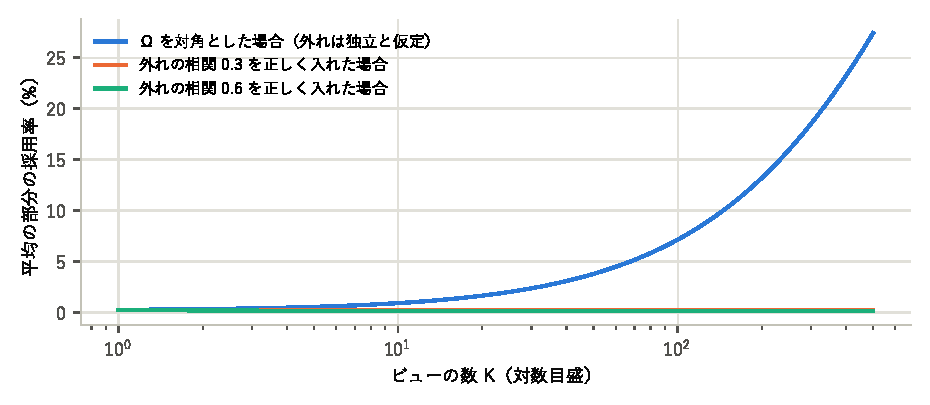
\includegraphics[width=0.92\linewidth]{fig_stack.pdf}
\caption{ビューの数と、平均の方向の採用率。外れが独立と仮定すると（青）、ビューが増えるほど全体の水準を強く信じる。外れの相関を正しく入れると（橙・緑）、採用率は増えない。}
\label{fig:stack}
\end{figure}

\tabref{tab:stack} と\figref{fig:stack} のとおり、外れの相関が 0.3 のとき、正しい採用率は $K$ によらず \V{stk.k500.true}\% だが、対角の $\Omega$ では $K=500$ で \V{stk.k500.diag}\% になる。100 倍以上の積み上がりである。

\section{本プロジェクトの外れの共通部分}

本プロジェクトの LLM の予想の外れ（予想 $-$ 翌月の実際）に、どれくらい共通の部分があるかを測った。判断日ごとの外れの平均の分散と、銘柄ごとの外れの分散の比から、等相関のモデルの $\rho_e$ を推定すると、約 \V{stk.rhoe} だった。外れの分散のうち、月ごとの共通の部分が占める割合は \V{stk.common.share}\% 程度である。

さらに、判断日ごとの予想の平均（LLM が見込む「全体の水準」）と、翌月の実際の平均の相関は \V{stk.level.corr} で、負だった。予想の平均の散らばり（日次 \V{stk.qlevel.sd}\%）は、実際の平均の散らばり（日次 \V{stk.rlevel.sd}\%）と同じくらいの大きさなのに、向きが合っていない。30 か月しかないので確かなことは言えないが、少なくとも「全体の水準の予想を数百倍に積み上げて信じる」根拠は、データにない。

\section{どう防ぐか}

\begin{enumerate}
\item \textbf{$\Omega$ を $\Sigma$ に比例させる}：$\Omega=\tau(1/s-1)P\Sigma P\T$（市場版なら $(1/s-1)P\Sigma P\T$）。外れの相関をリターンの相関と同じとみなす。どの方向にも採用率 $s$ がかかり、積み上がらない。本プロジェクトの計算（\chapref{ch:project}）の「$\Sigma$ に比例」の版である。
\item \textbf{全体の水準と差を分ける}：予想から判断日ごとの平均を引いて相対ビューにし、全体の水準は（入れるなら）別の 1 つのビューとして、それに見合う不確かさで入れる（\chapref{ch:shape}）。本プロジェクトのように全体の水準の予想が当たっていないなら、入れないのがよい。
\item \textbf{外れの共分散を推定する}：過去の外れから、共通の部分（ファクター）と個別の部分を推定し、$\Omega$ を「ファクターの構造」で作る。データが十分にあれば、もっとも正確である。
\end{enumerate}

\begin{keybox}[この章のまとめ]
\begin{itemize}
\item ビューの外れに共通の部分があるのに $\Omega$ を対角にすると、全体の水準への確信がビューの数に比例して積み上がる。例では、500 個のビューで採用率が 0.25\% から \V{stk.k500.diag}\% になった。
\item 外れの相関をリターンの相関と同じにする（$\Omega\propto\Sigma$）と、ビューの数によらず採用率は $\IC^2$ のままになる。
\item 銘柄間の差の予想は、全体の水準の予想より確かである。相対ビューにして、全体の水準は別に扱う。
\item 本プロジェクトの予想の外れの相関は約 \V{stk.rhoe} で、全体の水準の予想は翌月の実際と負の相関（\V{stk.level.corr}）だった。
\end{itemize}
\end{keybox}
